\chapter{Content Analysis}

Content analysis is a technique deployed by information architects for helping
them generate a sound and well structured website architecture. It consists of
two phases: collection of a representative sample of data and an analysis of
this content \citep[pp.~241--243]{morville06}.
A graphical content mapping can be included as an optional
intermediate phase between data inventory and analysis if one finds such
representations helpful for understanding a website's structure.
In it's essence a content analysis should identify the various
relationships (or lack of correlation) between a website's content items.
% all references needed

Instead of using content analysis as a means for improving on an existing
site's content architecture we'll be tailoring this technique to best help us
discover and understand social navigation patterns in infamous websites which
are known to make good use of such navigational designs. This means that we'll
concentrate only on core content objects and the relationships amongst them
which are organically generated---relationships which are made as part of
past users' behavior which can be leveraged by other users as a social form
of navigation.

The results of the low-level content inventories can be found in
Appendix~\ref{appendix:content.inventory}
(p.~\pageref{appendix:content.inventory}).
Particularly striking
samples from graphical content mappings will be sprinkled throughout the
subsequent analysis to illustrate certain findings. The content mappings in
their full glory are located in
Appendix~\ref{appendix:content.mapping}
(p.~\pageref{appendix:content.mapping}).

\section{Flickr}

Flickr is a photo sharing site which are known to be on the cutting edge when
it comes to enabling new and innovating navigational features. This subsequent
analysis of Flickr will be carried out as a registered user. One has to be
registered for interacting with the site in such a way that one leaves
persistent traces. The site has a open nature enabling anonymous access
to the majority of content.

\subsection{Thumbnails}

Already on the welcome page (Figure~\ref{figure:scrsh.flickr.welcome},
p.~\pageref{figure:scrsh.flickr.welcome})
we're finding navigation links that are social of
nature. Four thumbnails functions as sample of the most recently uploaded
photos by other members of the community. One can either navigate straight to
a detailed page for each particular photo by clicking on the respective
thumbnail (Id 6, p.~\pageref{table:flickr.content.inventory.6})
or the profile of the uploader by clicking on their user
name (Id 7, p.~\pageref{table:flickr.content.inventory.7}). Such thumbnails
with minimal meta data (the uploader) are prevalent all over Flickr. Of the
120 pages we collected in our content inventory 26 of them contained
thumbnails. Most of these thumbnails
are giving users incentives to navigate using social means%
\sidenote{Apart from the few pages that only show a
          stream of your own thumbnails--when you're browsing your
          own photos by various methods.}.
Which photos these thumbnails portray is dynamic. That is to say that other
users' actions--uploading a photo, tagging a photo, taking a photo with a
specific camera, collecting photos into sets, and adding photos to a certain
group--all determine the navigational choices you as a user is
presented with.
% maby connect this to thumbnail paper: cockburn06

\subsection{Meta-data}

\sidefill
\sidefigure{Flickr Photo Meta-data}{%
  Photo Meta-data,
  retrieved October 28, 2007, from
  \url{http://flickr.com/photos/benbengraves/187609810/}.
}{%
  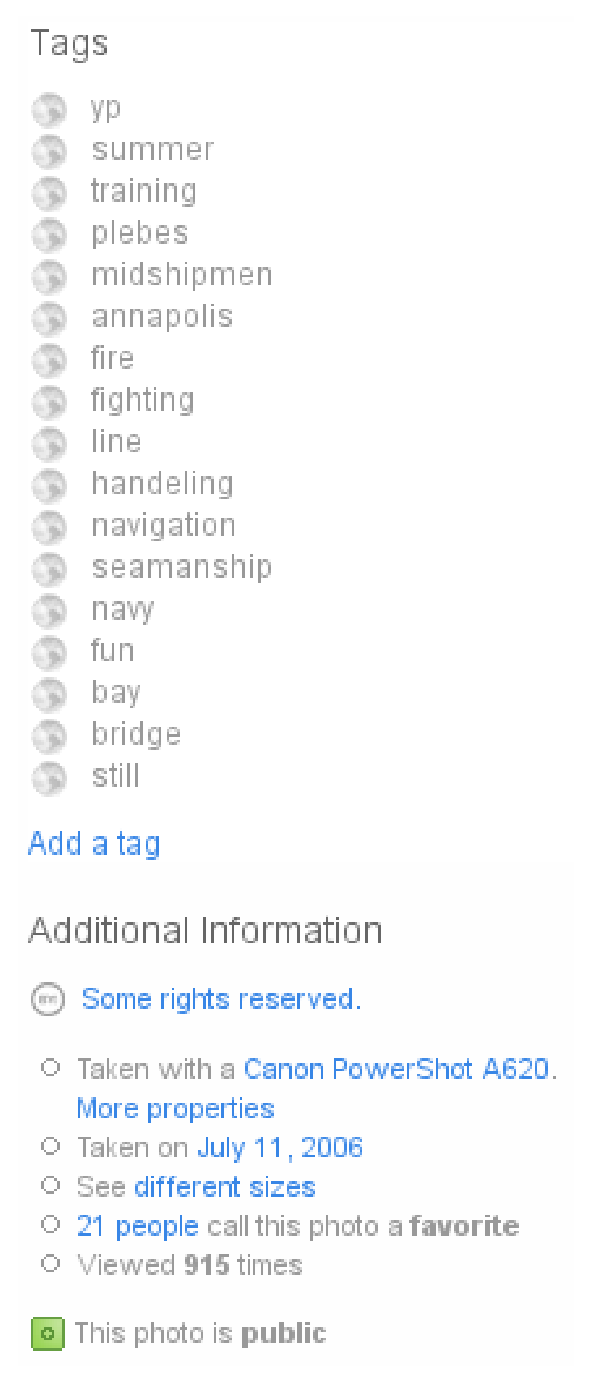
\includegraphics[width=\marginparwidth]{scrsh_flickr_photo_detail_metadata}
  \label{figure:scrsh.flickr.photo.detail.metadata}
}

We arrive on a photo detail page as in
Figure~\ref{figure:scrsh.flickr.photo.detail}
(p.~\pageref{figure:scrsh.flickr.photo.detail})
if we utilize one of these thumbnails for navigation. In addition to comments
on the photo we find meta-data as in 
Figure~\ref{figure:scrsh.flickr.photo.detail.metadata}
(p.~\pageref{figure:scrsh.flickr.photo.detail.metadata}).
Meta-data include the date the photo was taken, the manufacturer and the model
of the camera that was used which are all so called Exif%
\sidenote{Exchangeable Image File: a specification for image file format used
in digital cameras.}
data. Flickr utilize this data by enabeling navigation based both on the
dates a picture was taken and by camera make and model. Say you're trying to
find a picture from your home town on a particulary beautiful summer day. By
using date of picture taking based navigation coupled with tags or
geographical data (which both will be discussed shortly) you're probably
increasing you chances of finding what you want. Camera make information could
be useful when looking at the quality of pictures taken with certain cameras
before purchasing one yourself.

\subsection{Folksonomy}
% most important, basis for geo i early days with geo tagging and third party
% services (citation needed). Cite interview with co-founder about it's
% importance and findability it provides. Write about clustering, it's
% principles and what it provides. Cite when it was introduced.
Of most importance
for Flickr, and indeed what makes Flickr a folksonomy, is tags. Every
registered user can label anyone's photos by applying such short descriptive
tags. This collaborative process lay the ground work for other user's ability
to easily browse photos by topic.
Figure~\ref{figure:scrsh.flickr.tagcloud}
(p.~\pageref{figure:scrsh.flickr.tagcloud}) exemplifies how the user generated
data trough tagging can be used as a navigational aid. A so called \emph{tag
cloud} is used to visualize the popularity (and thereby importance) of the
individual tags. The larger the tag title, the more frequent the tag has been
in use.

Tagging is a very flexible approach only hindered by users' imagination. In the
early days of Flickr there was no support for geographical data. Users soon
found a remedy for this by tagging photos with longditude and latitude
(citation needed).

% Split into these sections:

\subsection{Geographical data}
In late August 2006 Flickr introduced geotagging abilities%
\sidenote{
  See
  \url{http://blog.flickr.com/en/2006/08/28/great-shot-whered-you-take-that/}
  for the announcement}.
By integrating
geographical aspects from Yahoo! Maps%
\sidenote{
  Available at \url{http://maps.yahoo.com}.
}
users could now place their photos on a
map to signify where they were captured. (TODO: finish geo description, take
screenhot, write about the unreleased ``places'' feature).
% Write about early geo tagging here. Write about the new places feature.
% Write and cite when proper geo data was incorporated.


\begin{figure}[b]
  \captionstyle{\raggedright}
  \centering
  \strictpagechecktrue
  \begin{adjustwidth*}{0em}{-\wholemargin}
    \begin{minipage}[t]{0.475\wholewidth}
      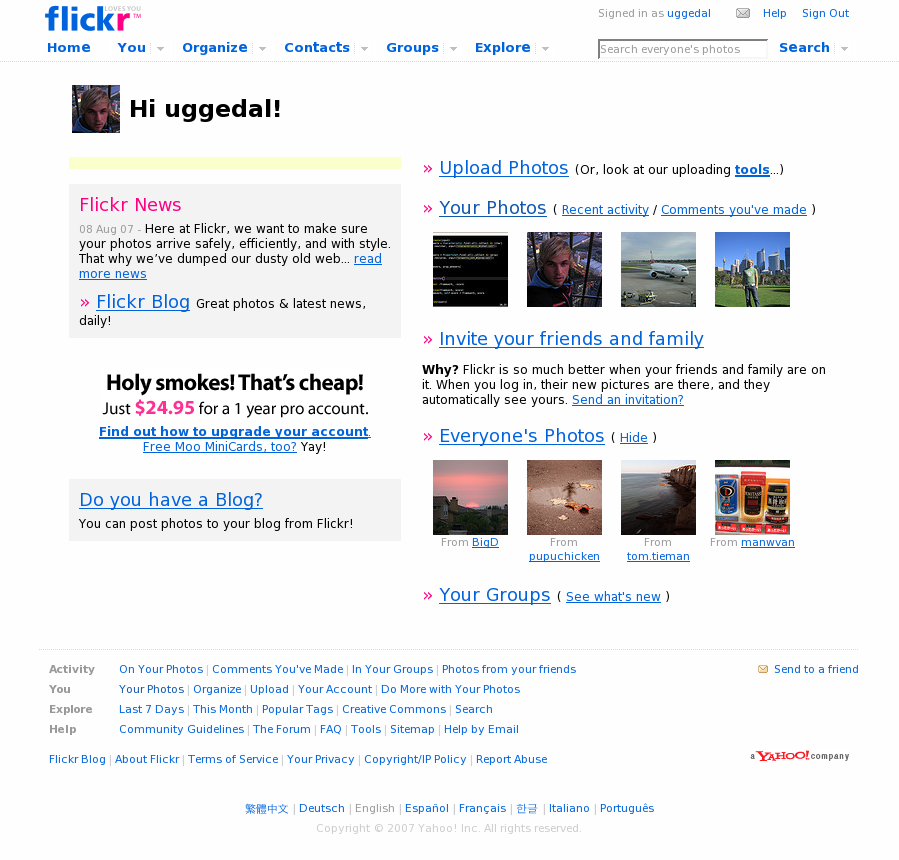
\includegraphics[width=\textwidth]{scrsh_flickr_welcome}
      \caption[Flickr Welcome Page]{%
         The Welcome Page,
         retrieved October 16, 2007, from \url{http://flickr.com}.}
      \label{figure:scrsh.flickr.welcome}
    \end{minipage}
    \hfill
    \begin{minipage}[t]{0.475\wholewidth}
      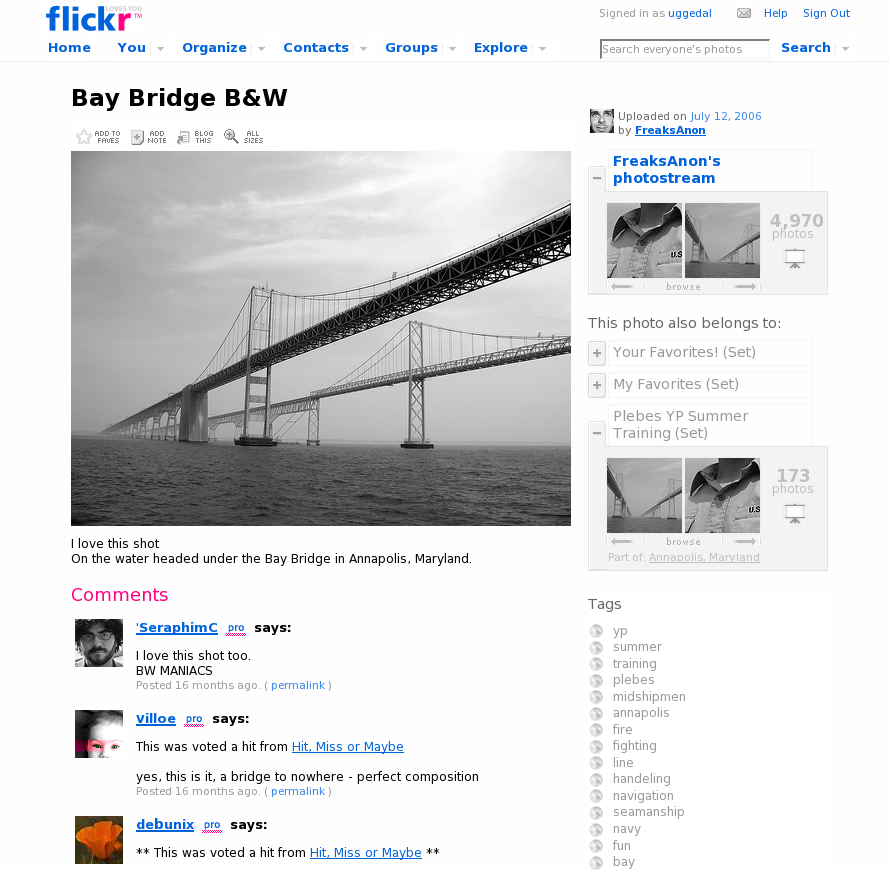
\includegraphics[width=\textwidth]{scrsh_flickr_photo_detail}
      \caption[Flickr Photo Detail Page]{%
         A Photo Detail Page,
         retrieved October 26, 2007, from
         \url{http://flickr.com/photos/benbengraves/187609810}.}
      \label{figure:scrsh.flickr.photo.detail}
    \end{minipage}
  \end{adjustwidth*}
  \normalcaption
\end{figure}

\begin{figure}
  \centering
  \strictpagechecktrue
  \begin{adjustwidth*}{0em}{-\wholemargin}
    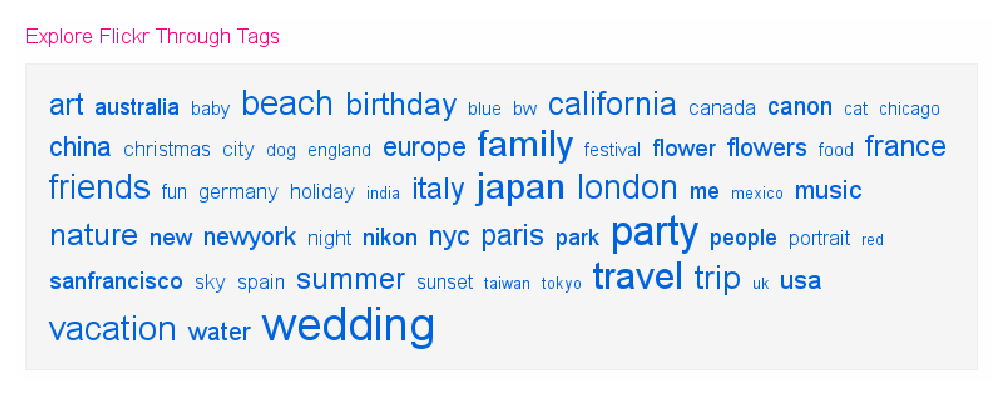
\includegraphics[width=\wholewidth]{scrsh_flickr_tagcloud}
    \caption[Flickr Tag Cloud]{%
       Tag Cloud,
       retrieved November 1, 2007, from \url{http://flickr.com/explore}.}
    \label{figure:scrsh.flickr.tagcloud}
  \end{adjustwidth*}
\end{figure}

